\documentclass[a4paper]{article}

\usepackage{INTERSPEECH2018}
\usepackage{cite}

\title{Paper Template for INTERSPEECH 2018}
\name{Dhruv Mishra}
%The maximum number of authors in the author list is twenty. If the number of contributing authors is more than twenty, they should be listed in a footnote or in acknowledgement section, as appropriate.
\address{
  IMS, University of Stuttgart}
\email{author@university.edu}

\begin{document}

\maketitle
%
\begin{abstract}
  This report describes the paper \cite{dredze2010nlp} which was presented by me and two other papers: \cite{li2018spoken} and \cite{rosiger2017improving}.
\end{abstract}

\section{NLP on spoken documents without ASR}
\subsection{Introduction}
The paper \cite{dredze2010nlp} describes a technique to apply NLP algorithms directly on spoken documents by transforming the speech data into a vector representation which is very similar to how textual data is represented. The motivation to do this are many:

\begin{itemize}
\item The current popular technique of using an ASR system to transcribe spoken documents is not very efficient. This method is prone to limitations imposed by the ASR system and error propagation into the entire pipeline.
\item Building an ASR system is very expensive and difficult to do. The training often requires a large amount of engineering knowledge, many hours of annotated audio data and machines for carrying out the computations.
\item ASR systems in general do not work across languages. Multi-lingual speech recognition models have been presented in the past but their accuracy is often quite less as compared to a monolingual ASR system.
\item Out of vocabulary terms is a bigger problem in ASR than text data, simply because of the size of the training data. For comparison, Switchboard corpus has about 1 million tokens whereas Common crawl has about 600 billion tokens. Therefore, it is highly likely that the number of unseen words will be far larger in speech data as compared to text data.
\item ASR accuracy will put an upper limit to the accuracy of the overall pipeline.
\item NLP algorithms applied on text data often use simple features like term frequency (tf), inverted document frequency (idf) etc. Requirement for annotations is often very minimal and these techniques work across different languages.
\item ASR systems on the other hand require a lot of annotated data, which is not always practical to procure or create.
\end{itemize}

Therefore, a technique to convert speech into an appropriate vector representation which can be used as input to NLP algorithms is presented. This is very similar to the idea of word embeddings, where text data is converted into vectors representations before they are fed into a machine learning algorithm.

\subsection{Data}
The paper uses a subset of the Switchboard Telephone Speech Corpus. This corpus has 2400 two sided telephone conversations on 70 pre-selected topics. The six most commonly topics were selected: \textbf{recycling, capital punishment, drug testing, family finance, job benefits, car buying}. For these topics, 60 sides of conversations were randomly selected. The resulting data set therefore contained 360 documents spoken by different speakers and was 36 hours in length.


\subsection{Architecture Overview}
The whole architecture has the following major components:

\begin{itemize}
\item Speech data: Raw speech data is taken from multiple speakers.
\item Dot Plot Matching: Acoustic dot plots using Posteriorgram representation are created to find matching regions.
\item Pseudo-terms: The matched regions are clustered together to form pseudo terms, which represent a word or a phrase in the document.
\item NLP: The pseudo terms are then used as an input for an NLP task. In this paper, topic classification of the spoken documents is performed.
\end{itemize}

\subsection{Dot Plots}
Dot plots is a method which has been borrowed from bio-informatics. Given character strings s1 and s2, substrings which are common to both of them can be seen as diagonal line segments in the visualisation. If the two strings are same, there will be a main diagonal which will be a result of self similarity. Therefore, search is for line segments other than the main diagonal to identify repetitions.

% \begin{figure}[t]
%   \centering
%   \includegraphics[width=\linewidth]{fig1.png}
%   \caption{An example of dotplot for the string "text processing vs speech processing" plotted against itself.}
%   \label{fig:dotplot}
% \end{figure}

\subsection{Posteriorgram Representations}
To adapt dot plots for spoken documents, the speech signals must be converted into a sequence of frames. Each frame is represented as the posterior probability distribution over a set of speech sounds given the speech observed at the particular point in time. The paper uses an English phone-set but it claims that it can be used for any language. The reason is that as long as the speech is reliably mapped to a probability distribution over this phone set, different languages will also get mapped into the same domain. This results in the applicability of this representation across different languages, although the paper does not test this hypothesis. This representation is also speaker-independent and provides sparsity to enable efficient storage and computation.

To illustrate this advantage, the authors state that they were able to perform the $O(n^2)$ dotplot computations for 60+ hours of speech (36 hours of training speech data matched with itself), which roughly corresponds to 500 terapixel of dotplots in approximately 5 hours using a grid of 100 cores.

\subsection{Acoustic Dot Plots}
Given a spoken document represented as a sequence of frames represented with posteriorgrams, an acoustic dotplot can be created, similar to the string dot plot where instead of matching characters, the frames are matched instead. This dot plot will have diagonal line segments for frames which are similar. The authors do not provide the details about the algorithm used for performing the dot plot matching, but it can be assumed to be trivial in the context of this work.

\subsubsection{Hyperparameters during matching phase}
While matching characters is a simple task of checking if the two characters are the same, matching frames is a more subjective problem. The paper proposes two parameters to determine what an acoustic match is:

\begin{itemize}
\item $\kappa$: This is the duration of the match in seconds.
\item $\tau$: The overlap threshold, i.e. the extent of similarity. A value of 1 is an exact match whereas 0.5 means only half of the frame is a match.
\end{itemize}

The paper presents the matching results by varying the values of both of these parameters simultaneously. Decreasing $\kappa$ results in more matched regions and increasing $\tau$ results in less frames getting matched. Both of them increase the number of pseudo-terms.

\subsection{Pseudo Terms}
Pseudo-terms represent a single word or phrase spoken at multiple points throughout the corpus. Each pseudo-term takes the place of a word of phrase in a bag or terms vector space model of a text document and allows the use of standard NLP algorithms. Pseudo-terms are created using by clustering the matched regions in the documents.

\subsubsection{Creating Pseudo-terms}
After finding a set of matched regions, graph clustering is used to aggregate the similar matches into a cluster.
The clusters thus formed are the pseudo-terms which represent a word of a phrase.

To take an example, suppose the phrase “It is sunny today” occurs once in three documents A,B and C. The acoustic dotplots will give three matches: AB, AC and BC. Each of these matches will have slightly different representations since the speakers are different. Using graph clustering, these matches are aggregated into a single cluster. This cluster is a pseudo-term which represents the term “It is sunny today” and has a tf of 3 and idf of 0 (because it occurs in 3 “documents”).

\subsubsection{Evaluation metrics for Clustering}
The clusters created by graph clustering were evaluated on three metrics:

\begin{itemize}
\item Purity: The precision of each cluster, i.e., how many examples in each cluster belong to the same true topic. Higher values are better.
\item Entropy: how the members of a cluster are distributed amongst the true labels. Lower values are better.
\item B-cubed: measures clustering effectiveness from the perspective of a user’s inspecting the clustering results. Directly quoting from the paper, "B-cubed precision can be defined as an algorithm as follows: suppose a user randomly selects a single example. She then proceeds to inspect every other example that occurs in the same cluster. How many of these items will have the same true label as the selected example (precision)?". Higher values are better.
\end{itemize}

\subsubsection{Clustering results}
The pseudo-terms created by graph clustering were compared with two other baseline methods: Phonetic Trigrams (three sequential phones) and Word Transcripts (Unigram, Bigram, Trigram). It must be noted that Word Transcript is the upper-bound for performance because in the best case, the pseudo-terms created will be the exact representations of words in the textual transcripts.

For each $\kappa$ the same narrow range of $\tau$ values achieve good results. The best result was for $\kappa$ = 0.6 s and $\tau$ = 0.96 which yielded a purity of 0.9750. The purity of unigram word transcript is 0.9917 whereas that of phonetic trigram is 0.6194. It must also be noted that decreasing $\kappa$ meant more features, but these additional features did not improve clustering performance in any measurable way. After performing clustering on the tuning and evaluation data, the final best values of the hyper-parameters was determined to be $\kappa$ = 0.7 s and $\tau$ = 0.98.

\subsection{Supervised Classification using pseudo-terms}
The pseudo-terms thus created were then used to do a topic classification task, where each document is labelled with the topic it belongs to. The topics were the six most common ones: recycling, capital punishment, drug testing, family finance, job benefits, car buying. Since the labels are balanced, random guessing will yield accuracy of 0.1667. A supervised learning algorithm was trained using labelled data and then asked to label some unseen test data.

The performance was evaluated on four popular learning algorithms:MIRA, Confidence Weighted (CW), Maximum Entropy, Support Vector Machines (SVM). In all four cases, the pseudo-term performance was quite close to the Word transcript performance and significantly better than Phonetic Trigrams.

The best performing configuration after performing the same selection heuristic as in clustering, was for $\kappa$ = 0.75 s and $\tau$ = 0.97. It is interesting to note that the parameter values are quite similar for the clustering and the classification task, which means that both of these two components are compatible with each to be used in a cascade setting. This detail is very important because it justifies the use of pseudo-terms. If the optimal parameters had been drastically different for the two stages, we would have two models which work very good on their own but perform badly together, something which is not the goal.

% \begin{figure}[t]
%   \centering
%   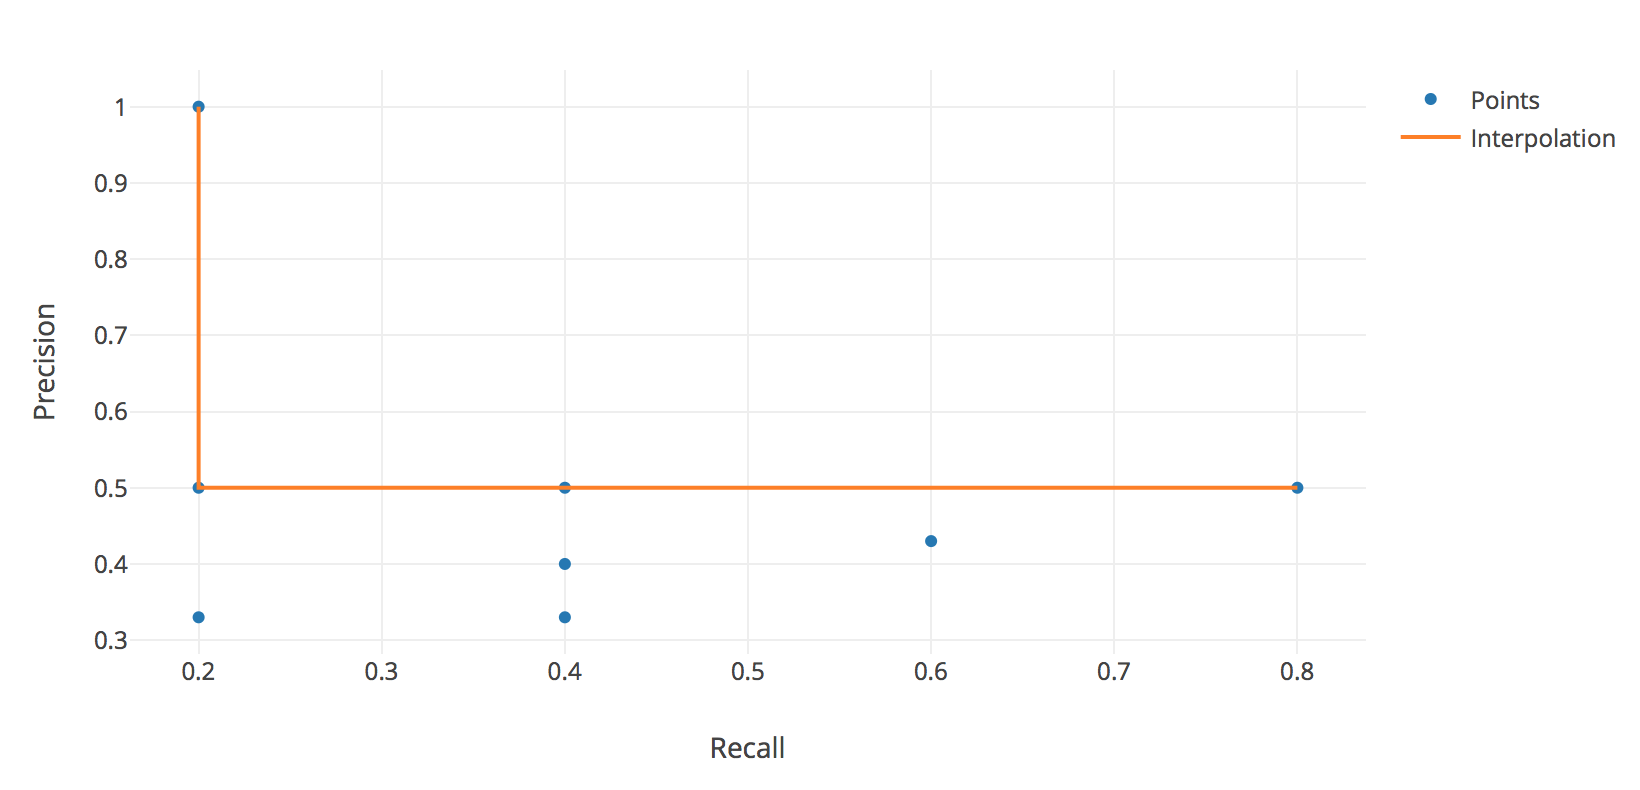
\includegraphics[width=\linewidth]{figure.pdf}
%   \caption{Schematic diagram of speech production.}
%   \label{fig:speech_production}
% \end{figure}

\subsection{Conclusions}
This paper presents a new strategy to perform unsupervised clustering and supervised classification of spoken documents by proposing a method to convert speech documents into a bag of words model of pseudo-terms and then using standard NLP algorithms. The performance is quite close to manual word transcriptions, which is the theoretical upper-bound and significantly exceeds that achieved with a phonetic recognizer.

\section{Spoken SQuAD: A Study of Mitigating the Impact of Speech Recognition Errors on Listening Comprehension}
\subsection{Introduction}
The primary motivation behind this work is the fact that humans can read plain-text documents faster than they can consume multimedia content. To put this fact in perspective, a normal reader who uses subvocalization, i.e. speaking each word internally in the mind (which is equivalent to hearing spoken version of the text) can read approximately 250 words per minute whereas, a reader who employs visual reading, i.e. understanding the meaning of the word without speaking it loud inside the mind or hearing it can read approximately 700 words per minute. Therefore, the idea of developing a machine to understand spoken documents is very appealing.

This paper uses the Stanford Question Answering Dataset (SQuAD) \cite{rajpurkar2016squad}, which is a popular Question Answering (QA) corpus and converts it into a speech processing task by converting the text documents into speech documents with the help of Google Text-to-Speech software. This new task, which takes a spoken reference document and a question in text form to answer it using the document is named as Spoken Question Answering (SQA). The authors then evaluate the effect of the ASR system analyzing the document and propose various measures to mitigate the impact of ASR error on the overall system.

\subsection{Task Description}
\subsubsection{Corpus}
All of the text documents in SQuAD are converted into speech documents. The answer to each question is a span of the document. The entire corpus was randomly partitioned into 80\% training, 10\% development and 10\% test. The speech documents were then transcribed into text using CMU Sphinx. The questions were left in their original textual form. Answers which were not present in the ASR transcriptions were removed due to their non-triviality.

\subsubsection{Evaluation Metrics}
The authors propose two ways to evaluate the model:

\begin{itemize}
  \item Directly compute the Exact Match (EM) and F1 scores between the predicted text answer and the ground-truth text answer. If the predicted text answer and the ground-truth text answer are exactly the same, then the EM score is 1, otherwise 0

  \item  compute Audio Overlapping Score (AOS) between the time span of system output and the ground-truth time span as $AOS = (X \cap Y)/(X \cup Y)$. Here, X is the audio time of predicted answer and Y is the audio time of ground truth answer. To calculate audio time, the timestamp of every word is used.
\end{itemize}

\subsection{Model}
The SQA is a cascade of an ASR module and a Reading Comprehension module.

\subsubsection{Reading Comprehension Models} \label{rcmodels}
The various Reading Comprehension models which have shown to have good performance on SQuAD are: BiDirectional Attention Flow (BiDAF), R-NET, Mnemonic Reader, FusionNet and Dr.QA.

\subsubsection{Subword units and Phoneme CNN}
Subword units are smaller parts of a word. They can be of many types: characters, phonemes or syllables. These units can provide important additional information to the reading comprehension module because as is very often the case, an ASR system might correctly transcribe parts of word even then the complete word was transcribed incorrectly.

The authors train word embeddings by training a CNN on a input subword sequence, similar to the usual method of applying CNN on a sequence of character for text data. The parameters of the embedding matrix are learned end-to-end with the reading comprehension module during the same training process.

\subsection{Experimental Results}

\subsubsection{Impact of ASR Errors}
The various models listed in \ref{rcmodels} were trained on SQuAD training set and tested on SQuAD dev set and Spoken SQuAD test set. EM and F1 both drastically reduced in the test set. No AOS scores were provided.

\subsubsection{Training on ASR transcripts}
The models BiDAF and Dr.QA were trained on training sets of both SQuAD and Spoken SQuAD and tested on test set of Spoken SQuAD. The results showed that the models trained on Spoken SQuAD achieved better EM and F1 scores in the presence of ASR errors in the test data.

\subsubsection{Mitigating ASR errors with Subword Units}
Each word was converted into a sequence of phonemes using the CMU LOGIOS Lexicon Tool, which was then fed into the Phoneme CNN to create word embeddings. Five different configurations were tried out: Word, Word+Char, Word+Phoneme, Word+Syllable and Word+Char+Phoneme+Syllable.

The embeddings were then used with BiDAF and the results showed that Word+Char+Phoneme+Syllable setting achieved the best performance over both the evaluation metrics. However, with the addition of a dropout layer in Phoneme CNN, the Word+Phoneme embeddings gave the best results.

\subsubsection{Analysis}
The results showed that BiDAF with only word embeddings is not robust to ASR errors but the addition of phoneme sequence embeddings results in the selection correct answers despite ASR errors.

\subsection{Conclusion}
This paper presented a new task description for evaluating the answering capabilities of a machine when the reference documents are present in speech format. This task which is currently dependent on an ASR transcribing module is greatly limited in it's performance by the errors introduced by ASR. A technique of phonetic embeddings was proposed to mitigate these errors, but the overall performance is still significantly lagging behind that of traditional text based QA systems.

\section{Improving coreference resolution with automatically predicted prosodic information}
\subsection{Introduction}
Coreference resolution refers to grouping the Noun Phrases referring to the same entity in a text or spoken document. This paper presents a method to automatically predict pitch accents using the acoustic features extracted from the speech signal and adding this information to the text features such as POS tags and other syntactic information used by a coreference resolver. The reason to do is because it has been observed that using text features on spoken documents leads in a drop in performance. Prosody is useful because it provides two important signals: firstly, it can help in distinguishing between already known and new information. Secondly, in spoken language, there is a tendency for the coreferent phrase to be not have any accent.

\subsection{Prosodic Features} \label{prosodicfeatures}
A pilot study done by \cite{rosiger2015using} showed the usability of pitch accents and prosodic phrasing where these features were added to the usual text based features. However, the pitch accents were added manually and this is not a very scalable method. Therefore, the authors of this paper (\cite{rosiger2017improving}) try to automate this process of adding pitch accents by predicting them directly from the acoustic features of the speech signal. Two labels were defined to use pitch accents:

\begin{itemize}
  \item Short NPs: uses the absence of a pitch accent.
  \item Long NPs: nuclear accents are more relevant as their presence indicates that the NP is less likely to be a part of a reference chain.
\end{itemize}

The features which were demonstrated to be useful in the pilot study are Pitch accent presence and Nuclear accent (derived from phrase boundary) presence. They were calculated for every NP.

\subsection{Data}
The DIRNDL dataset was used in this paper. It is a German radio news corpus having manual coreference and prosody labels. The documents were spoken by 13 male and 7 female speakers and the total length of audio was approximately 5 hours. The two features described in \ref{prosodicfeatures} were used as the class labels for automatic prediction.

\subsection{Automatic Prosodic information}
\subsubsection{Model} \label{model}
A model is a CNN which takes an input word and it's right and left adjacent word as the context window. The input matrix is a frame based representation of speech and the output is a boolean value denoting the presence or absence of pitch the prosodic event. The signal is divided into overlapping frames of length 20ms with a shift window of 10ms. Each frame is represented by a 6 dimensional feature vector. Therefore, the input matrix is a concatenation of three frames. The acoustic features used were: smoothed fundamental frequency (f0), RMS energy, PCM loudness, voicing probability and Harmonics-to-Noise Ratio. The model has two convolution layers followed by a max-pool layer.

\subsubsection{Prosodic labels for DIRNDL corpus}
The CNN model for detecting prosodic events is trained on an English corpus and tested on the German corpus. The english dataset used for training is a 2.5 hour subset of the Boston University Radio News Corpus and it contains manually annotated prosodic labels. The reason to use an English dataset here was to avoid the use of the same German language data twice. If the german data is being used to train prosodic labels and then again in the training of coreference resolution, the complete model pipeline is very prone to over-fitting.

The performance on the German corpus for both the events mentioned in \ref{prosodicfeatures} is over 80\%. Therefore, it can be inferred that training over english corpus is also applicable to german corpus and the model can be used along with the coreference resolver.

\subsection{Coreference Resolution}
The IMS HotCoref DE was used as the coreference resolver in this paper. The baseline used in this paper is this model trained on the concatenation of training and development data of the DIRNDL corpus. The score achieved is 46.11.

\subsection{Experiments and Analysis}
The prosodic features trained from \ref{model} are added to the feature set of the baseline resolver. This setting is tested on three configurations:

\begin{itemize}
  \item trained and tested on manual prosodic labels (gold).
  \item trained on manual prosodic labels, but tested on automatic labels (gold/auto).
  \item trained and tested on automatic prosodic labels (auto).
\end{itemize}

Two different configurations of feature sets were used for each of the above mentioned variations: Short NPs (NPs of length less than 3) and All NPs. Therefore a total of 6 different configurations were tested.

The performance for the coreference resolver was improved as compared to the baseline by the addition of prosodic event (pitch accent or nuclear accent) in all the configurations. As expected, the pattern of gold>gold/auto>auto was observed for both Short NPs and All NPs, which tells us that the errors in the CNN model are being propagated here. However, the difference between gold and auto was very marginal for all NPs in pitch accent detection and Short NPs in nuclear accent detection whereas the difference was much larger for the other cases.

Pitch accent was more informative for Short NPs because Long NPs are accented most of the time. On the other hand, Nuclear accent is more informative for Long NPs as compared to Short NPs, but it improved performance over baseline in both cases.



\subsection{Conclusion}
The paper showed a process to automatically predict prosodic labels. Although the predicted labels were not as accurate as the gold labels, their addition still resulted in an improved performance by the coreference resolver. This result supports the fact that prosodic information is helpful and further work to extract better labels from auditory features will improve performance of coreference resolution too. As future work, the authors suggest the use of ASR transcriptions instead of gold text transcriptions and adding lexical or syntactic information to the prosodic label predictor.

\bibliographystyle{IEEEtran}

\bibliography{mybib}

% \begin{thebibliography}{9}
% \bibitem[1]{Davis80-COP}
%   S.\ B.\ Davis and P.\ Mermelstein,
%   ``Comparison of parametric representation for monosyllabic word recognition in continuously spoken sentences,''
%   \textit{IEEE Transactions on Acoustics, Speech and Signal Processing}, vol.~28, no.~4, pp.~357--366, 1980.
% \bibitem[2]{Rabiner89-ATO}
%   L.\ R.\ Rabiner,
%   ``A tutorial on hidden Markov models and selected applications in speech recognition,''
%   \textit{Proceedings of the IEEE}, vol.~77, no.~2, pp.~257-286, 1989.
% \bibitem[3]{Hastie09-TEO}
%   T.\ Hastie, R.\ Tibshirani, and J.\ Friedman,
%   \textit{The Elements of Statistical Learning -- Data Mining, Inference, and Prediction}.
%   New York: Springer, 2009.
% \bibitem[4]{YourName17-XXX}
%   F.\ Lastname1, F.\ Lastname2, and F.\ Lastname3,
%   ``Title of your INTERSPEECH 2018 publication,''
%   in \textit{Interspeech 2018 -- 19\textsuperscript{th} Annual Conference of the International Speech Communication Association, September 2-6, Hyderabad, India Proceedings, Proceedings}, 2018, pp.~100--104.
% \end{thebibliography}

\end{document}
